
\chapter{Experiments}
\label{chapter:experiments}


\section{Performance comparison of practical examples}
\label{section:exp_seissol_star}

The goal of the first experiment is to show that the general approach can yield a speedup on matrices which are of practical interest. In the case of SeisSol, the compute kernels are recursively nested matrix multiplications of the pattern $Q' \mathrel{{+}{=}} K \cdot Q \cdot A$, where $K$ and $A$ are sparse and $Q$ is dense. The $A$ matrix always has the same shape and sparsity pattern, whereas there are many different matrices shaped like $K$. The performance of various kernels on the $Q \cdot A$ multiplication is depicted in Figure~\ref{fig:perf_seissol}. 

Unfortunately, the case of the $K \cdot Q$ multiplication can not be simply plugged in to SeisSol due to the asymmetry between dense and sparse multiplication discussed in Section~\ref{section:asymmetry}. However, if the dense matrices were stored in row-major format instead of column-major, the situation would be reversed. Because the $K$ matrix is larger, this might yield a greater speedup on SeisSol as a whole. For these reasons the transposed problem $Q \cdot K$ is also considered in Figure~\ref{fig:perf_seissol_K}.


The experimental setup is straightforward. The problem size is set as $m=40,~n=15,~k=9$, corresponding to a viscoelastic rheological model as described in~\cite{7568431}. The sparsity pattern used is shown on the right in Figure~\ref{fig:seissol_star}. The only variable measured is wall clock time, which was used to calculate speedup relative to \py{libxsmm}'s dense kernel. The two new kernels tested are UnrolledSparse and GeneralSparse. The only available degree of freedom for matrices this small is the $m$-block size; the two extremes, $bm=8$ and $bm=40$, were both considered. The TiledSparse and BlockSparse kernels, on the other hand, were not considered because they would either degenerate to UnrolledSparse or produce complete fill-in, depending on the chosen block sizes $bn, bk$. The performance of Breuer's sparse kernels was also tested for comparison. 



  \begin{figure}[!htb]
    \centering
%    \begin{subfigure}[b]{0.4\textwidth}
%      \centering
      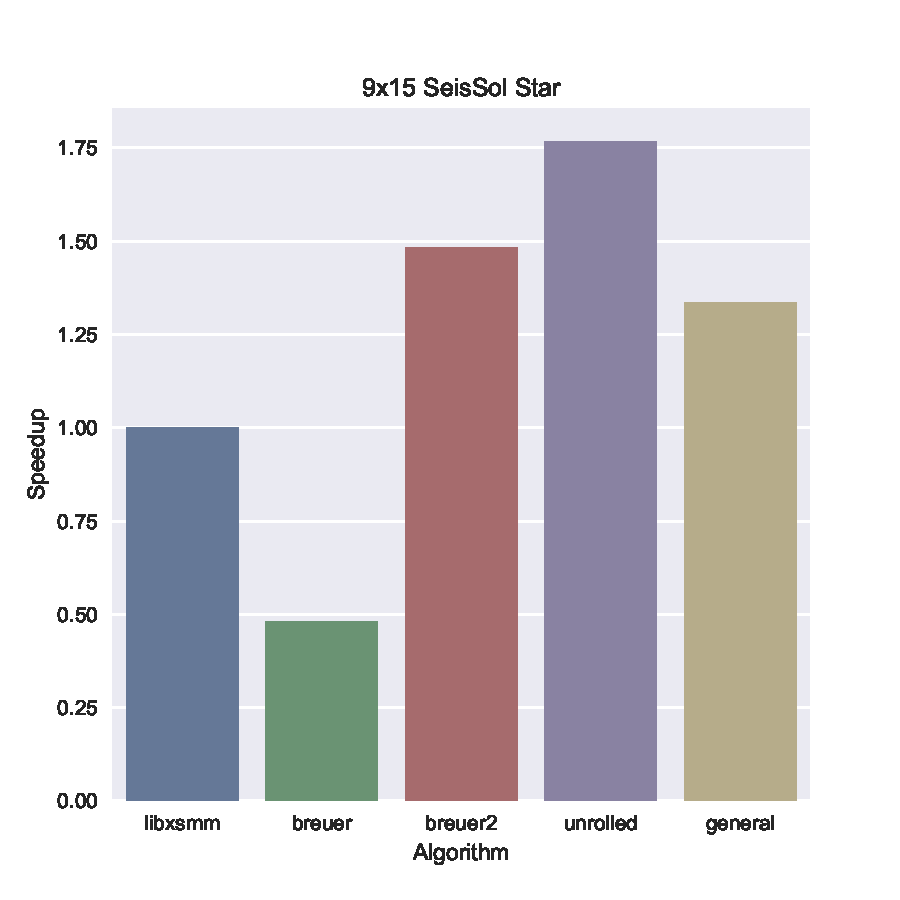
\includegraphics[width=0.75\textwidth]{images/seissol_comparison.pdf}
      \caption{Performance comparison of different spgemm kernels for the 9x15 SeisSol `star' matrix}
      \label{fig:perf_seissol}
%    \end{subfigure}
  \end{figure}


The experiment shows that the UnrolledSparse kernel with $bm=8$ has the best performance, corresponding to a speedup of $1.83$ over dense. To put this in context, the upper bound on the speedup for this problem is $(n\cdot k)/nnz = 3.97$. The UnrolledSparse with the larger block size performs slightly worse, at $1.74$. The GeneralSparse with the larger block size performed similarly worse than its UnrolledSparse equivalent, which was expected due to the indirect jump penalty. Meanwhile, the GeneralSparse with the small block size experienced a slowdown. 

The automatically generated Breuer kernel also experienced a slowdown relative to dense, which was not surprising considering the architectural disadvantages it is working against. However, an examination of the code revealed a bug: the SIMD vector length was being constrained to 32 bytes instead of 64. Manually fixing this led to a speedup of almost $1.5$ over dense, significantly better but still less than the UnrolledSparse kernel. The performance of the modified Breuer is expected to be similar for small matrices but then diverge as they get larger and denser, due to Breuer's lack of an accumulator for blocks of $C$. 

This experiment can be repeated for different patterns of $K$, and also for the $A$-matrix sizes $n \in \{27, 36\}$. 


\section{Scaling of UnrolledSparse}
\label{section:exp_unrolled_scaling}

The goal of this experiment is to determine the range of problems which benefit from UnrolledSparse, and examine how its performance varies over this range. The focus is on matrix density rather than matrix size. UnrolledSparse is expected to have an upper limit on the number of nonzeros in B, and it is desirable to find this limit experimentally. Below it, the amount of computation is expected to scale according to $2\cdot m \cdot nnz$, but because this also reduces the arithmetic intensity, it remains to be seen how the time to solution scales.

The experimental setup is as follows. The matrix sizes are taken to be $m=128, n=28, k=128$, and they are blocked according to $bm=8, bn=28, bk=4$. These numbers were chosen to try to match the blocking behavior of \py{libxsmm}. The B matrix uses CSC format and is filled with a varying number of nonzeros. Time-to-solution is measured and the achieved FLOP/S rate is calculated.

  \begin{figure}[!htb]
    \centering
    \begin{subfigure}[b]{0.8\textwidth}
      \centering
      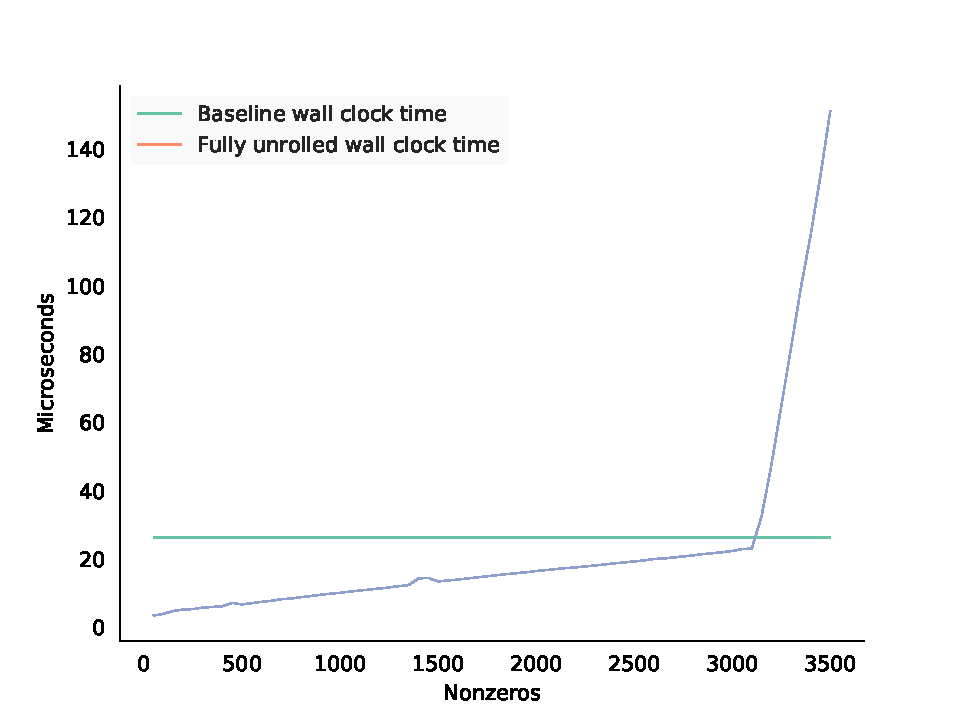
\includegraphics[width=\textwidth]{images/fig2.pdf}
      \caption{Time to solution for unrolledsparse}
      \label{fig:unrolled_time}
    \end{subfigure}
    \begin{subfigure}[b]{0.8\textwidth}
      \centering
      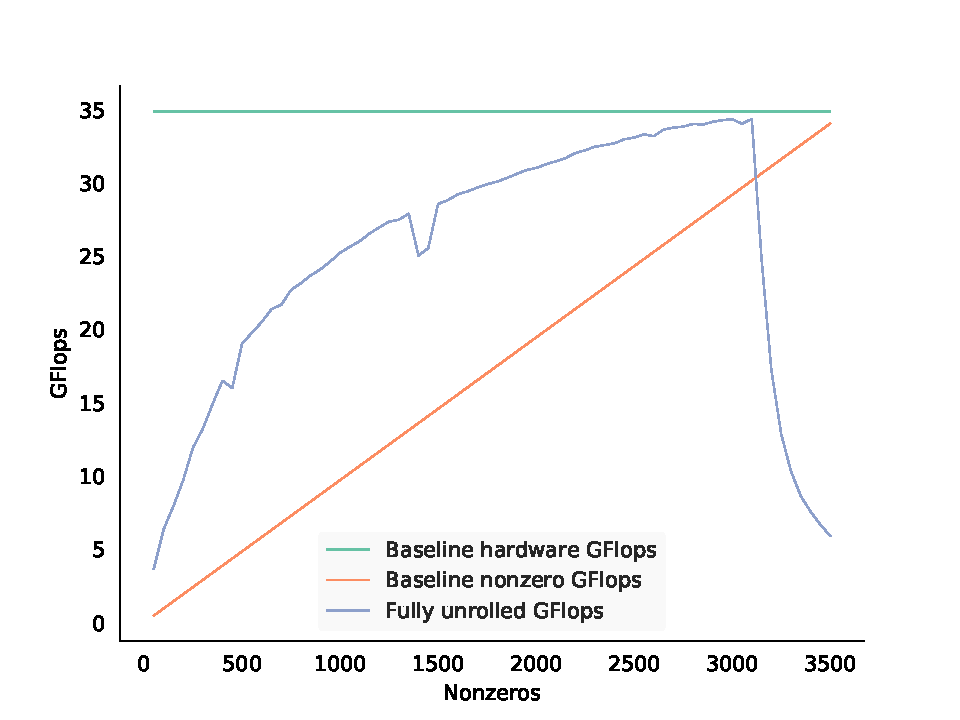
\includegraphics[width=\textwidth]{images/fig3.pdf}
      \caption{Performance of unrolledsparse}
      \label{fig:unrolled_perf}
    \end{subfigure}
  \end{figure}

  \begin{itemize}
    \item For $nnz < 3100$, time-to-solution scales linearly.
    \item For $nnz > 3200$, the FMAs completely fill the instruction cache (regardless of matrix dimensions!)
    \item Fully unrolled sparse algorithm outperforms dense ``nonzero'' GFlops, but always underperforms dense ``hardware'' GFlops
    

    Linear relationship between nnzs and time, with a constant offset compared to dense.

  \end{itemize} 



\section{Choice of block sizes}
\label{section:exp_unrolled_sizing}

The previous section demonstrated the utility of UnrolledSparse kernel, and also showed that the choice of block sizes $bm,bn,bk$ affects the overall performance. The KNL architecture places a number of constraints on the optimal block size, which is described in depth for the dense case by~\ref{Heinecke:2016:LAS:3014904.3015017}. The goal of this experiment is to test the performance of UnrolledSparse for different block sizes and see to what extent the empirical sparse results match with the theoretical dense analysis. This can also lead to heuristics for automatically choosing the block sizes.

For the experimental setup, we chose $m=n=k=96$ because it has a lot of convenient divisors and it is relatively large. This not only reduces measurement noise, but also stresses the data cache and possibly the instruction cache. Two cases were considered, $nnz=500$ and $nnz=2000$. The sparsity pattern was generated from a uniform random distribution. Kernels were generated for every choice of $bm \in \{8,16,24,32\}$ and $bn, bk \in \{1,2,3,4,6,8,12,16,24\}$ satisfying the MicroSparse constraint $(bk+bn) \cdot (bm/8) \leq 32$. 

The speedups of each kernel relative to dense are shown in Figure~\ref{fig:unrolled_sizing}. For $nnz=500$, the theoretical max speedup is $18.4$ and the observed max speedup is $6.57$, implying an efficiency of $0.36$. Meanwhile, for $nnz=2000$, the theoretical speedup is $4.61$ and observed is $2.96$, an efficiency of $0.64$. This is good news: not only did the efficiency \emph{improve} as more nonzeros were added, but the best speedup happened at similar block sizes. The next step is to understand these block sizes.

The first observation is that for any choice of $(bm, bn)$, the performance is effectively independent of $bk$. This makes sense because the unrolled $Bk$ loop is the innermost, so the choice of $bk$ ultimately only affects the ordering of \glspl{FMA} instructions, relative to loads of columns of A, within the same panel. Inefficiencies here can be resolved by the reorder buffer. \py{libxsmm} approaches this differently: instead of unrolling a $Bk$ loop of arbitrary size, it tackles the entire panel at once, keeping the current block of A in a ring buffer of 2-4 registers, and manually scheduling its load operations. An earlier experiment suggested that the choice of scheduling did not strongly affect performance, so the ring buffer approach was abandoned in favor of the conceptually simpler block unrolling.

The second observation is that the best choice of $bn$ is directly tied to $bm$. For now consider only the $nnz=500$ case. The maxima happen at $(bm,bn) \in \{(8,16), (16,4), (24,2)\}$, and decrease as $bm$ increases. Thus $bm=8$ is preferred as long as the matrix dimensions support a tiling where $bn \in \{12,16\}$. Otherwise a tiling with $bm=16, bn\in\{1,2,3,4\}$ is better. 

This is consistent with libxsmm, which abandoned their 2D blocking of C ($16 \times 3$) in favor of a 1D blocking ($8 \times 30$) specifically for \gls{KNL}. They argue that the movement of columns of A into registers needs to be minimized relative to the number of FMAs in that block because of the narrow out-of-order execution issue width discussed earlier. Some of this reasoning applies to UnrolledSparse, since a smaller $bn$ 

Now let's turn to the $nnz=2000$ case. The pattern looks similar for $bm=8, bn\in\{8,12,16,24\}$, but becomes qualitatively different for all $bm > 8$ or $bn < 6$. This is a plane in the problem space, beyond which performance falls off a cliff. 


  \begin{figure}[tb]
    \centering
    \begin{subfigure}[b]{0.45\textwidth}
      \centering
      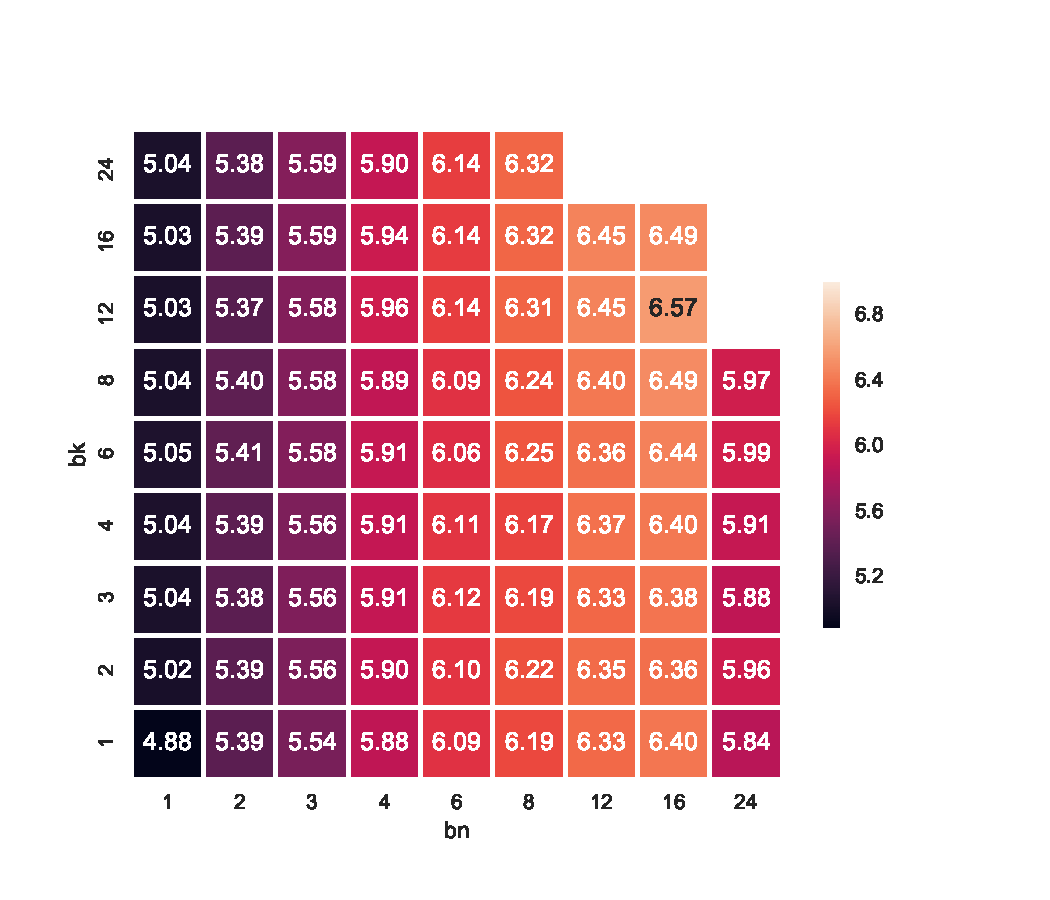
\includegraphics[width=\textwidth]{images/unrolled_sizing_500_8.pdf}
      \caption{bm = 8, nnz = 500}
    \end{subfigure}
    \begin{subfigure}[b]{0.45\textwidth}
      \centering
      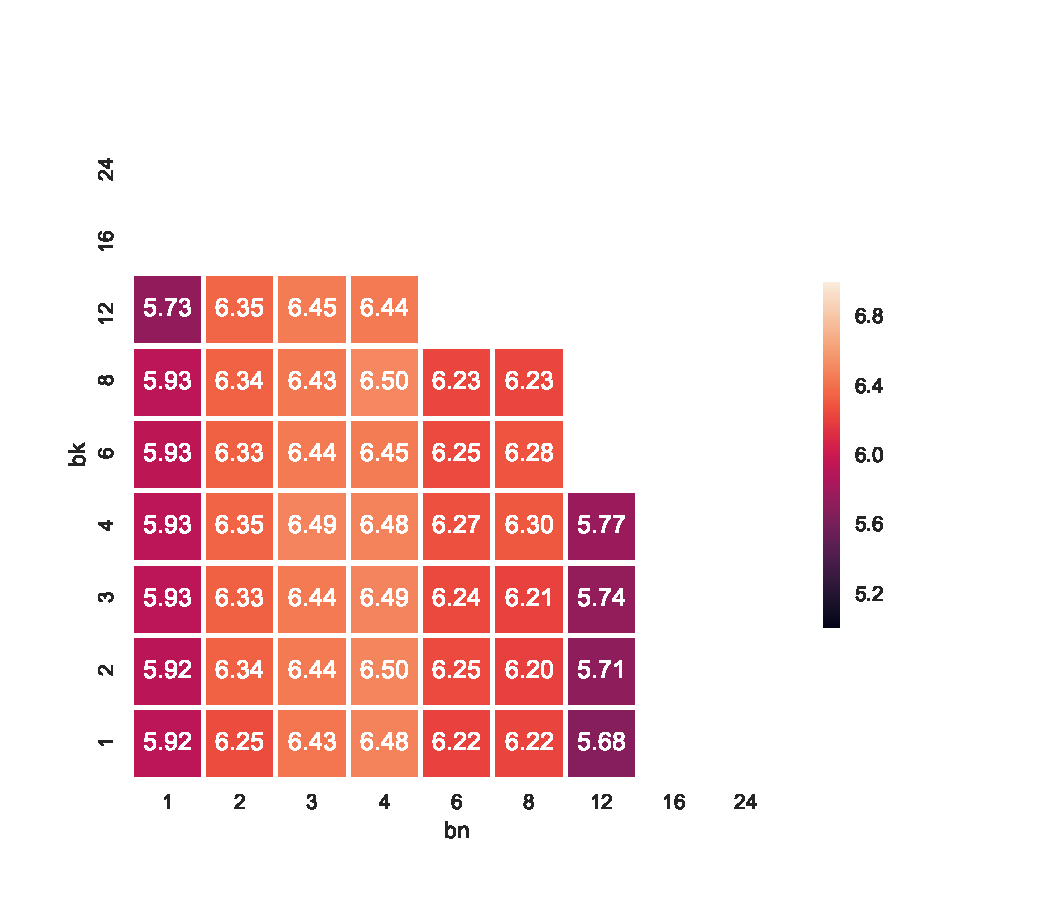
\includegraphics[width=\textwidth]{images/unrolled_sizing_500_16.pdf}
      \caption{bm = 16, nnz = 500}
    \end{subfigure}
    \begin{subfigure}[b]{0.45\textwidth}
      \centering
      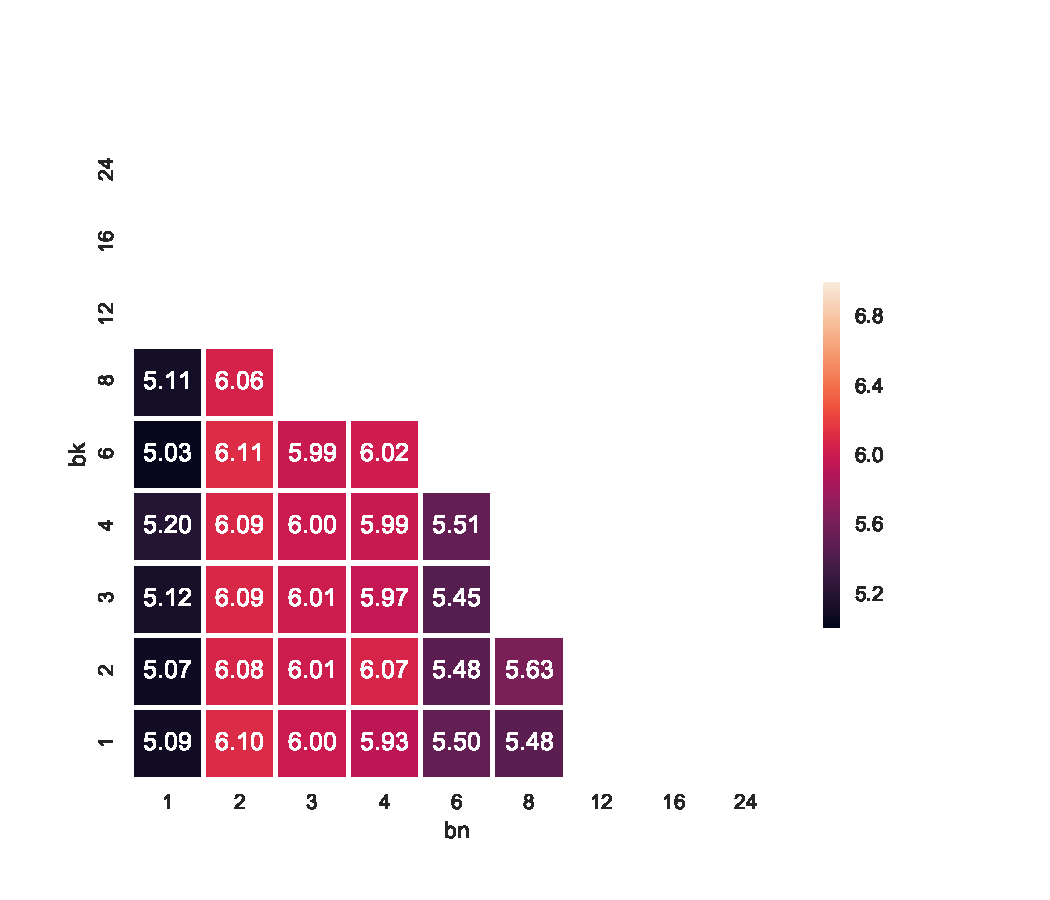
\includegraphics[width=\textwidth]{images/unrolled_sizing_500_24.pdf}
      \caption{bm = 24, nnz = 500}
    \end{subfigure}
    \begin{subfigure}[b]{0.45\textwidth}
      \centering
      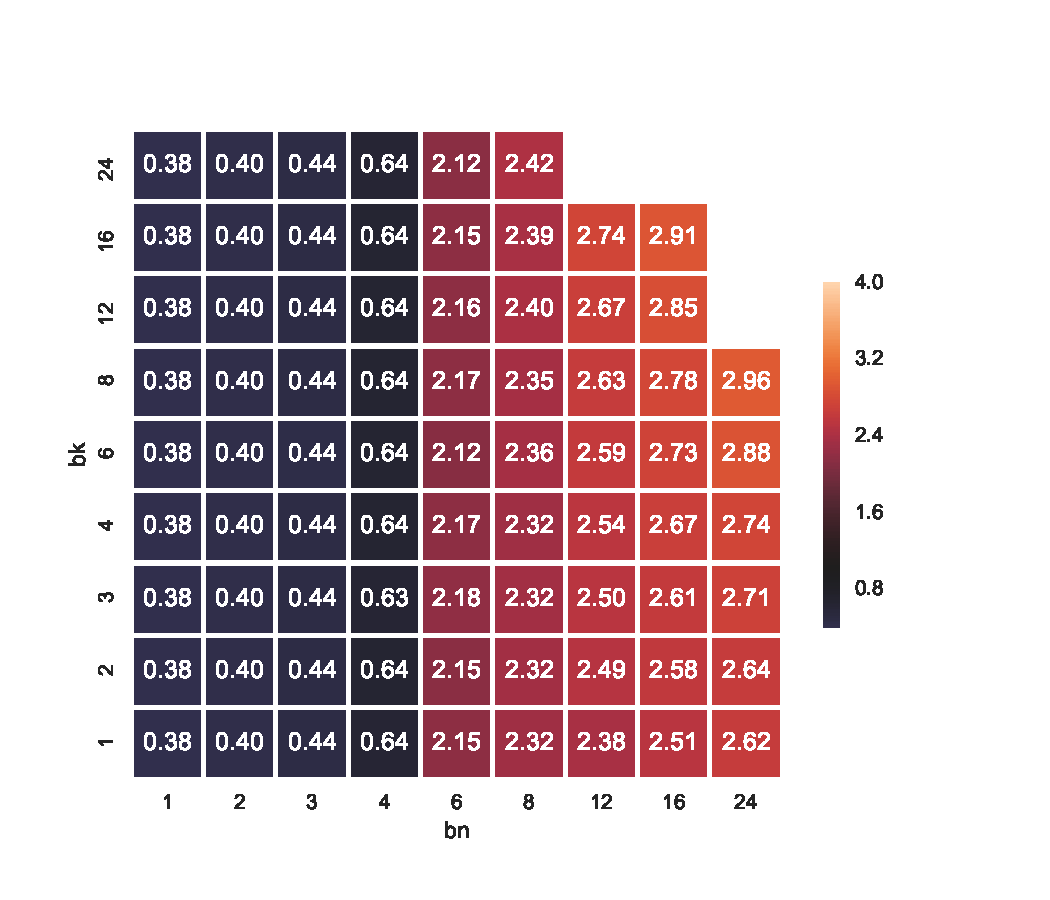
\includegraphics[width=\textwidth]{images/unrolled_sizing_2000_8.pdf}
      \caption{bm = 8, nnz = 2000}
    \end{subfigure}
    \caption{Speedup of a $96 \times 96$ random sparse matrix with different choices of block size. For smaller $nnz$, the speedup varies smoothly, every choice yields a speedup, and simple heuristics can be derived. For larger $nnz$, there are performance cliffs at $bn < 6$ and $bm > 8$.}
    \label{fig:unrolled_sizing}
  \end{figure}


\section{Performance of GeneralSparse}
\label{section:exp_jump_scaling}


  \begin{figure}[!htb]
    \centering
    \begin{subfigure}[b]{0.8\textwidth}
      \centering
      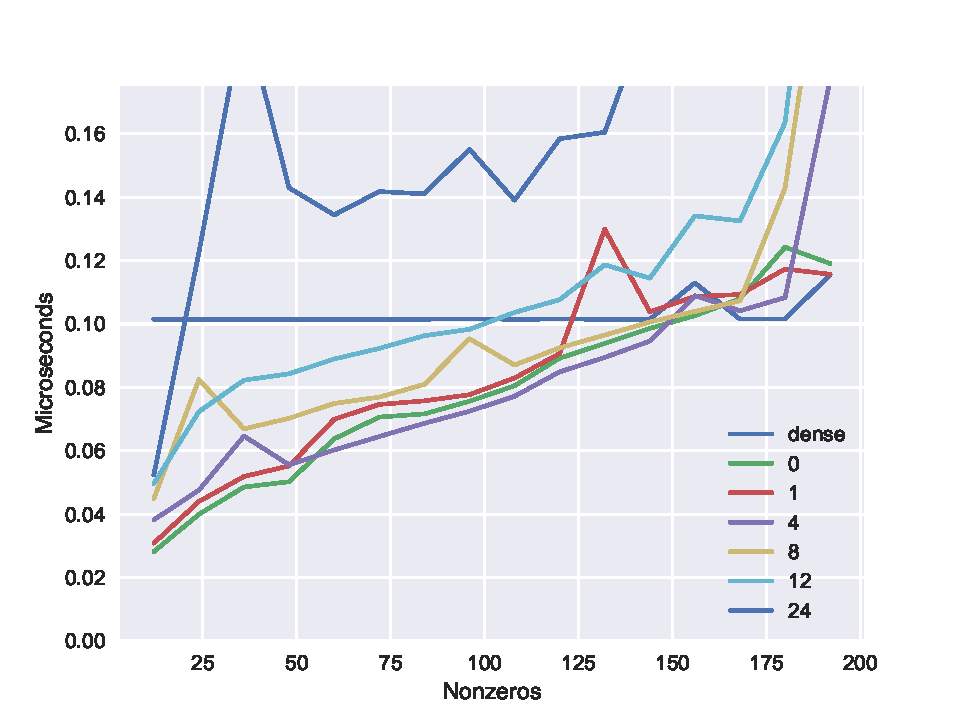
\includegraphics[width=\textwidth]{images/jump_penalty.pdf}
      \caption{Small-scale }
      \label{fig:unrolled_time}
    \end{subfigure}
    \begin{subfigure}[b]{0.8\textwidth}
      \centering
      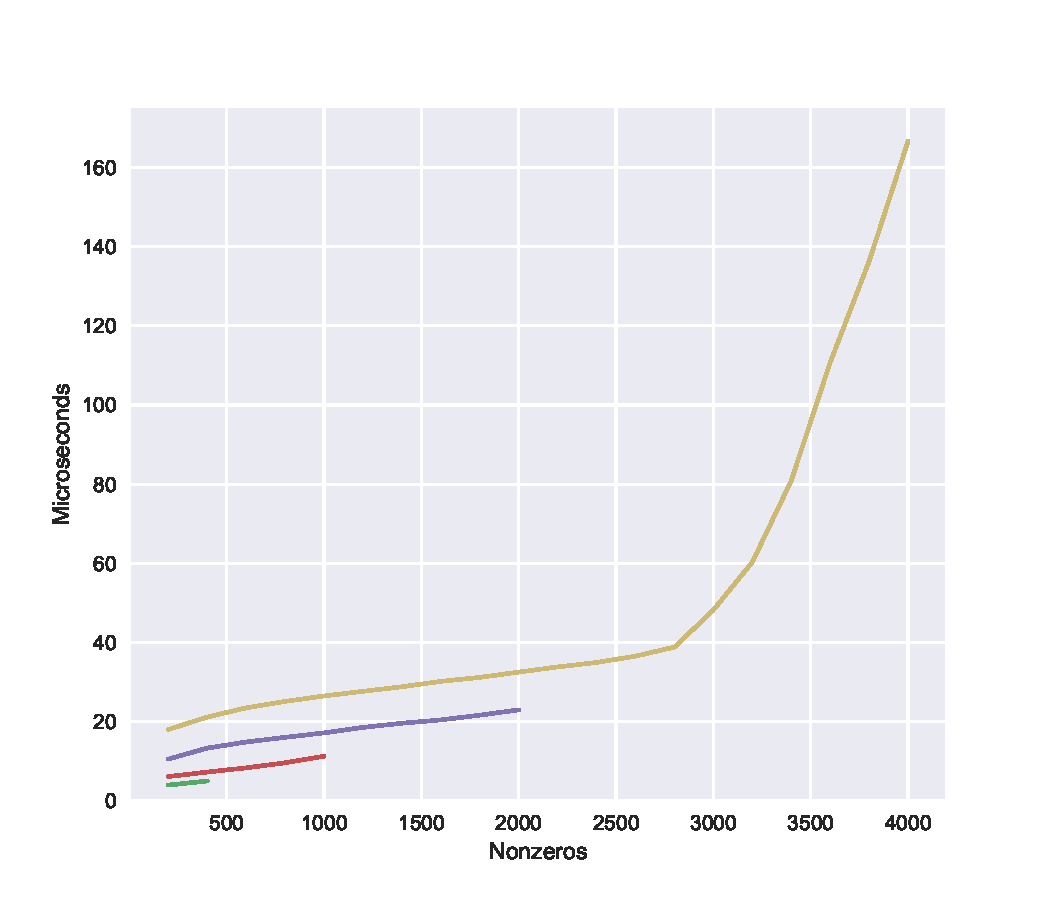
\includegraphics[width=\textwidth]{images/jump_scaling.pdf}
      \caption{Large-scale performance}
      \label{fig:unrolled_perf}
    \end{subfigure}
  \end{figure}



